\chapter{確率 - Probability}

\index{確率 - probability}

\key{確率 - probability}は0から1の間の実数で表されるある事象がどの程度の確率で起こるかを示すものです。
ある事象が確実に起こるなら確率は1であり、確実にあり得ないならその確率は0です。
ある事象の確率は$P(\cdots)$と表記され、3つの点がその事象を表します。

サイコロを投げるとき、その結果は1から6の整数であり、それぞれの結果が出る確率は1/6です。
このため、次のような確率が計算できる。

\begin{itemize}[noitemsep]
\item $P(\textrm{''4がでる''})=1/6$
\item $P(\textrm{''6以外''})=5/6$
\item $P(\textrm{''偶数''})=1/2$
\end{itemize}

\section{確率の計算 - Calculation}


ある確率を計算するには組合せ論を用いるか、その事象が発生する過程をシミュレートする方法があります。
シャッフルした山札から同じ数字のカードを3枚引く確率を計算してみます。(例えば、$\spadesuit 8$, $\clubsuit 8$, $\diamondsuit 8$)。

\subsubsection*{方法1}

次の式を使うことができます。

\[\frac{\textrm{望ましい数量}}{\textrm{あり得る全体の数}}.\]

この問題では、各カードの価値は同じです。
このような結果は,$13 {4 \choose 3}$あります。
ある数を引く可能性は 13パターンがあり、
その中で4つのスーツのうちから3つを引くのは
${4 \choose 3}$のパターンがあります。
ここで全体の引くパターンは52枚のカードから3枚のカードを選ぶので、
${52 \choose 3}$です。
この確率は以下の様になります。

\[\frac{13 {4 \choose 3}}{{52 \choose 3}} = \frac{1}{425}.\]

\subsubsection*{方法2}

今度はプロセスをシミュレ ーションするアプローチを考えます。
この例では、3枚のカードを引くので、3回のプロセスを実行します。
まず、1枚目のカードは何を選んでも良いです。
第2段階は51枚のカードが残っていて、そのうち3枚が最初のカードと同じ数なので$3/51$の確率で成功です。
3番目のステップも$2/50$の確率で成功です。つまり、全体の処理が成功する確率は以下の様になります。

\[1 \cdot \frac{3}{51} \cdot \frac{2}{50} = \frac{1}{425}.\]

\section{事象 - Events}

確率における事象は集合として表現できます。
\[A \subset X\]
$X$はすべての可能な結果全体で、$A$は結果の部分集合です。
サイコロを振るとその結果は
\[X = \{1,2,3,4,5,6\}\]
となり、''偶数である''という集合は以下の通りです。
\[A = \{2,4,6\}\]

ある事象$x$には確率$p(x)$が割り当てられています。
ある事象Aの確率P(A)は、次ように結果の確率の総和として計算することができます。
\[P(A) = \sum_{x \in A} p(x).\]
サイコロを投げる場合、各結果$x$に対して$p(x)=1/6$であるから、
''偶数である''という事象の確率は以下の通りです。
\[p(2)+p(4)+p(6)=1/2.\]

$X$の確率は1、つまり$P(X )=1$です。
各事象は集合なので標準的な集合演算で操作できます。

\begin{itemize}
\item \key{補集合 - complement} $\bar A$ は
''$A$ が起こらない''という意味です。
例えばサイコロにおいて、$A=\{2,4,6\}$の補集合は
$\bar A = \{1,3,5\}$です。
\item \key{集合和 - union} $A \cup B$ は
''$A$ か $B$ が起きる''という意味です。
$A=\{2,5\}$と$B=\{4,5,6\}$の和は、
$A \cup B = \{2,4,5,6\}$です。
\item \key{集合積 - intersection} $A \cap B$は
''$A$ と $B$ が起きる''という意味です。
$A=\{2,5\}$ と $B=\{4,5,6\}$の集合積は
$A \cap B = \{5\}$です。
\end{itemize}

\subsubsection{補集合 - Complement}

補集合$\bar A$は次の様に計算できます。
\[P(\bar A)=1-P(A).\]

補集合によって、ある問題の逆を解くことで簡単に解けることがあります。
サイコロを10回投げたとき、少なくとも1回6が出る確率は次の様に簡単に求められます。
\[1-(5/6)^{10}.\]

ここで、$5/6$は一投の結果が$6$でない確率です。
$(5/6)^{10}$は10投のうちただの一回も1投も6でない確率となります。そのため、これの補数が問題の答えとなります。

\subsubsection{集合和}

$A \cup B$の確率は以下の様に示ます。
\[P(A \cup B)=P(A)+P(B)-P(A \cap B).\]
例えば、サイコロを考えて、
\[A=\textrm{''偶数である''}\]
と
\[B=\textrm{''4未満である''}\]
であるとき、
\[A \cup B=\textrm{''偶数であるか4未満である''},\]
という確率は、
\[P(A \cup B) = P(A)+P(B)-P(A \cap B)=1/2+1/2-1/6=5/6.\]

となります。事象$A$と$B$が\key{不連続,排他的 - disjoint}、すなわち$A \cap B$が空である場合は事象$A \cup B$の確率は、単純に以下の様に示ます。

\[P(A \cup B)=P(A)+P(B).\]


\subsubsection{条件付き確率 - Conditional probability}

\index{条件付き確率 - conditional probability}

\key{条件付き確率 - conditional probability}
\[P(A | B) = \frac{P(A \cap B)}{P(B)}\]
というのは$B$が起こったと仮定した場合の$A$の確率でです。
したがって$A$の確率を計算するときは$B$に属する結果だけを考えます。
先ほどのセットを使うと、
\[P(A | B)= 1/3,\]
となります。Bの結果は$\{1,2,3\}$で、そのうちの1つは偶数だからです。
つまり結果が$1 \ldots 3$となった場合の偶数の結果の確率です。

\subsubsection{共通部分 - Intersection}

\index{独立 - independence}

条件付き確率を用いると共通部分である
$A \cap B$の確率は以下の様に求めることができます。
\[P(A \cap B)=P(A)P(B|A).\]
$A$と$B$が\key{独立 - independent}なのは次のときです。
\[P(A|B)=P(A) \hspace{10px}\textrm{かつ}\hspace{10px} P(B|A)=P(B),\]

ということは$B$が起こっても$A$の確率は変わらず、その逆も同様ということです。
さて、この場合に共通部分の確率は
\[P(A \cap B)=P(A)P(B).\]
です。例えば山札からトランプを引く場合に
\[A = \textrm{''スーツがクラブである''}\]
\[B = \textrm{''数字が4である''}\]
は独立です。このため、
\[A \cap B = \textrm{''クラブの4である''}\]
という確率は次の様に示ます。
\[P(A \cap B)=P(A)P(B)=1/4 \cdot 1/13 = 1/52.\]

\section{確率変数 - Random variables}

\index{確率変数 - random variable}

\key{ランダムな値 - random variable} はランダムに生成される値のことです。
例えば、2回サイコロを投げるときの考えられる確率変数は
\[X=\textrm{''出た目の和''}.\]

例えば結果が$[4, 6]$(最初に4で次に6だったという意味)であれば、$X$ の値は10とします。

例えば、2つのサイコロを投げるときに$P(X=10)=3/36$です。
結果の総数は36であり合計10を得るには$[4,6]$, $[5,5]$, $[6,4]$という3通りの可能性があるからです。

\subsubsection{期待値 - Expected value}

\index{期待値 - expected value}

\key{期待値 - expected value} $E[X]$ 確率変数 $X$ の平均値を示します。期待値は,以下の和として計算できます。
\[\sum_x P(X=x)x,\]
$x$は$X$でありうる全ての数です。

例えばサイコロを投げるときの期待値は以下の通りです。
\[1/6 \cdot 1 + 1/6 \cdot 2 + 1/6 \cdot 3 + 1/6 \cdot 4 + 1/6 \cdot 5 + 1/6 \cdot 6 = 7/2.\]

期待値の面白い性質は\key{線形性 - linearity}です。
$E[X_1+X_2+\cdots+X_n]$
は常に
$E[X_1]+E[X_2]+\cdots+E[X_n]$.
と等しいです。
この式は、確率変数が互いに依存しあっていても成り立ちます。

例えば、2つのサイコロを投げるとき期待される和は以下の通りです。
\[E[X_1+X_2]=E[X_1]+E[X_2]=7/2+7/2=7.\]

$n$個のボールが$n$個の箱にランダムに入れられて空箱の期待個数を計算する問題を考えます。
各球は等しい確率でどの箱にも入ります。$n = 2$の場合,次の様に考えられます。
\begin{center}
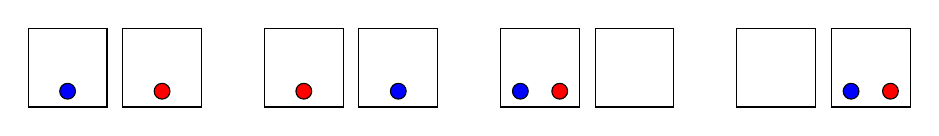
\begin{tikzpicture}
\draw (0,0) rectangle (1,1);
\draw (1.2,0) rectangle (2.2,1);
\draw (3,0) rectangle (4,1);
\draw (4.2,0) rectangle (5.2,1);
\draw (6,0) rectangle (7,1);
\draw (7.2,0) rectangle (8.2,1);
\draw (9,0) rectangle (10,1);
\draw (10.2,0) rectangle (11.2,1);

\draw[fill=blue] (0.5,0.2) circle (0.1);
\draw[fill=red] (1.7,0.2) circle (0.1);
\draw[fill=red] (3.5,0.2) circle (0.1);
\draw[fill=blue] (4.7,0.2) circle (0.1);
\draw[fill=blue] (6.25,0.2) circle (0.1);
\draw[fill=red] (6.75,0.2) circle (0.1);
\draw[fill=blue] (10.45,0.2) circle (0.1);
\draw[fill=red] (10.95,0.2) circle (0.1);
\end{tikzpicture}
\end{center}
このとき、空の箱の数は以下の通りです。
\[\frac{0+0+1+1}{4} = \frac{1}{2}.\]
一般に1つの箱が空の確率は、
\[\Big(\frac{n-1}{n}\Big)^n,\]
で求められます。その箱にボールが入っていないからです。
ここで線形性を利用すると期待値は次の様になります。
\[n \cdot \Big(\frac{n-1}{n}\Big)^n.\]

\subsubsection{分布 - Distributions}

\index{分布 - distribution}

\key{分布 - distribution}とは$X$が持ちうる各値の確率を示します。
分布は、値 $P(X=x)$ から構成されます。
2つのサイコロを投げるとき、その和の分布は次のようになります。

\begin{center}
\small {
\begin{tabular}{r|rrrrrrrrrrrrr}
$x$ & 2 & 3 & 4 & 5 & 6 & 7 & 8 & 9 & 10 & 11 & 12 \\
$P(X=x)$ & $1/36$ & $2/36$ & $3/36$ & $4/36$ & $5/36$ & $6/36$ & $5/36$ & $4/36$ & $3/36$ & $2/36$ & $1/36$ \\
\end{tabular}
}
\end{center}

\index{一様分布 - uniform distribution}
\key{一様分布 - uniform distribution}では確率変数$X$は$n$個の値 $a,a+1,\ldots,b$を取る時、
各値を取る確率は$1/n$とします。
サイコロをに当てはめれば$a = 1, b = 6$で、各値 $x$ に対して$P(X = x) = 1/6$です。
この様な一様分布における$X$の期待値は
\[E[X] = \frac{a+b}{2}.\]

\index{二項分布 - binomial distribution}
\key{二項分布 - binomial distribution}において、$n$回の試行があった時、
1回の試行が成功する確率を$p$とすると、確率変数$X$は試行の成功回数を数ることになります。
つまり、ある値$x$の確率は次のとおりです。
\[P(X=x)=p^x (1-p)^{n-x} {n \choose x},\]
ここで$p^x$と$(1-p)^{n-x}$はそれぞれ成功と失敗に対応しています。
${n \choose x}$はその試行が選ばれる回数です。

例えばサイコロを10回投げ、6が3回出る確率は、
$(1/6)^3 (5/6)^7 {10 \choose 3}$です。

二項分布における$X$の期待値は次の通りです。
\[E[X] = pn.\]

\index{幾何分布 - geometric distribution}
\key{幾何分布 - geometric distribution}とは、
試行が成功する確率を$p$とし、最初の成功が起こるまで続けます。
確率変数$X$は必要な試行回数を数えるもので、ある値$x$の確率は以下のとおりです。
\[P(X=x)=(1-p)^{x-1} p,\]
先ほどと同様に$(1-p)^{x-1}$は失敗した試行に対応し$p$は最初の成功した試行に対応します。

ここでサイコロを6が出るまで振るとして、投げた回数がちょうど4回である確率は
$(5/6)^3 1/6$となります。

幾何分布における$X$の期待値は次の通りです。
\[E[X]=\frac{1}{p}.\]

\section{マルコフ連鎖 - Markov chains}

\index{マルコフ連鎖 - Markov chain}

\key{マルコフ連鎖 - Markov chain}は状態とその間の遷移からなるランダムなプロセスのことです。
ここで各状態から他の状態に移行する確率は定義されています。
マルコフ連鎖は状態をノードとして遷移をエッジとするグラフで表現することができます。


次のような問題を考えます。
最初$n$階建ての建物の1階にいます。
各ステップにおいてランダムに1階上か1階下に移動します。
ただし、1階からは上にしか$n$階からは下にしかいけないとします。
さて、$k$歩いた後に$m$階にいる確率は?

この問題はマルコフ連鎖の1つで$n=5$の場合にグラフは以下のようになる。

\begin{center}
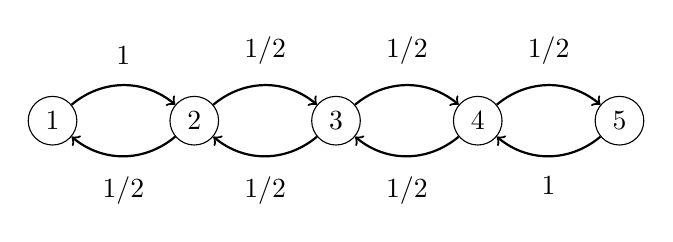
\begin{tikzpicture}[scale=0.9]
\node[draw, circle] (1) at (0,0) {$1$};
\node[draw, circle] (2) at (2,0) {$2$};
\node[draw, circle] (3) at (4,0) {$3$};
\node[draw, circle] (4) at (6,0) {$4$};
\node[draw, circle] (5) at (8,0) {$5$};

\path[draw,thick,->] (1) edge [bend left=40] node[font=\small,label=$1$] {} (2);
\path[draw,thick,->] (2) edge [bend left=40] node[font=\small,label=$1/2$] {} (3);
\path[draw,thick,->] (3) edge [bend left=40] node[font=\small,label=$1/2$] {} (4);
\path[draw,thick,->] (4) edge [bend left=40] node[font=\small,label=$1/2$] {} (5);

\path[draw,thick,->] (5) edge [bend left=40] node[font=\small,label=below:$1$] {} (4);
\path[draw,thick,->] (4) edge [bend left=40] node[font=\small,label=below:$1/2$] {} (3);
\path[draw,thick,->] (3) edge [bend left=40] node[font=\small,label=below:$1/2$] {} (2);
\path[draw,thick,->] (2) edge [bend left=40] node[font=\small,label=below:$1/2$] {} (1);

%\path[draw,thick,->] (1) edge [bend left=40] node[font=\small,label=below:$1$] {} (2);
\end{tikzpicture}
\end{center}

マルコフ連鎖の確率分布はベクトル$[p_1,p_2,\ldots,p_n]$ で
$p_k$は現在の状態が$k$である確率です。この時$p_1+p_2+\cdots+p_n=1$は常に成立します。

上記のシナリオでは最初は1階にいるので初期分布は $[1,0,0,0,0]$ です。
次の瞬間フロア1からフロア2にしか移動できないので、次の分布は$[0,1,0,0,0]$です。
この後は1階上か1階下に移動できるので次の分布は$[1/2,0,1/2,0,0]$となり、以下同様です。

これをシミュレーションする効率的な方法は、動的計画法 です。
各ステップで、どのように動くことができるかのすべての可能性を調べていけば、$m$ステップの歩みを $O(n^2 m)$ 時間でシミュレートすることができる。

また、この遷移は確率分布を更新する行列として表現することもできます。
\[
 \begin{bmatrix}
  0 & 1/2 & 0 & 0 & 0 \\
  1 & 0 & 1/2 & 0 & 0 \\
  0 & 1/2 & 0 & 1/2 & 0 \\
  0 & 0 & 1/2 & 0 & 1 \\
  0 & 0 & 0 & 1/2 & 0 \\
 \end{bmatrix}.
\]

確率分布にこの行列を掛けると、1ステップ移動した後の新しい分布が得られます。
例えば、分布$[1,0,0,0,0]$から分布$[0,1,0,0,0]$は次の通りです。

\[
 \begin{bmatrix}
  0 & 1/2 & 0 & 0 & 0 \\
  1 & 0 & 1/2 & 0 & 0 \\
  0 & 1/2 & 0 & 1/2 & 0 \\
  0 & 0 & 1/2 & 0 & 1 \\
  0 & 0 & 0 & 1/2 & 0 \\
 \end{bmatrix}
 \begin{bmatrix}
  1 \\
  0 \\
  0 \\
  0 \\
  0 \\
 \end{bmatrix}
=
 \begin{bmatrix}
  0 \\
  1 \\
  0 \\
  0 \\
  0 \\
 \end{bmatrix}.
\]

行列の累乗を効率的に計算することで$m$ステップ後の分布を$O(n^3 \log m)$で計算することができます。

\section{乱択}

\index{乱択}

問題を解くために確率とは関係ない問題だとしても、ランダム性を利用することがあります。
\key{乱択}はランダム性を用いたアルゴリズムです。

\index{モンテカルロ法(Monte Carlo algorithm)}

\key{モンテカルロ法(Monte Carlo algorithm)} は
間違った答えとなる可能性を十分に持つランダム化アルゴリズムです。
このアルゴリズムが適切であるためには、間違った答えが出る確率が十分に小さいことが必要です。

\index{ラスベガス法(Las Vegas algorithm)}

\key{ラスベガス法}は、間違った答えを出さないが、実行時間はランダムに変化するアルゴリズムである。
このアルゴリズムのデザインには効率的なアルゴリズムの設計が必要です。

ランダム性を利用して解くことができる3つの例題を紹介します。

\subsubsection{k番目に小さい数(Order statistics)}

\index{k番目に小さい数(Order statistics)}

配列の\key{k番目に小さい数(Order statistics)}は
昇順にソートした後の位置kにある要素です。
ですが、ある1つの要素を見つけるためだけに配列全体をソートする必要があるのでしょうか?
配列をソートせずにランダムなアルゴリズムでこれを求めることができます.
これは\key{quickselect}\footnote{In 1961,
C. A. R. Hoare published two algorithms that
are efficient on average: \index{quicksort} \index{quickselect}
\key{quicksort} \cite{hoa61a} for sorting arrays and
\key{quickselect} \cite{hoa61b} for finding order statistics.}
アルゴリズム、別名ラスベガス・アルゴリズムと呼ばれ、その実行時間は通常$O(n)$、最悪の場合$O(n^2)$です。

このアルゴリズムは配列のランダムな要素$x$を選び$x$より小さい要素を配列の左に、
それ以外の要素を配列の右側に移動させます.
これは要素がn個とすると$O(n)$で実行できます。
左側には$a$個の要素,右側には$b$個の要素があるとしましょう。
$a = k$ならば,要素$x$はk番目に小さい数です。
$a > k$の時は左側部分の$k$番目の数を再帰的に求め,
$a < k$の時は右側部分の$r$番目の数$(r = k - a)$を再帰的に求め,
要素が見つかるまで同様の方法で探索を見つければ良いのです。

$x$ がランダムに選ばれるため,配列のサイズは各ステップで約半分と期待できるので時間計算量は次のようになります。
\[n+n/2+n/4+n/8+\cdots < 2n = O(n).\]

最悪の場合は$O(n^2)$です。
これは$x$ が配列の最小または最大の要素の1つになるように常に選択される場合で$O(n)$ ステップが必要になるからです.
その確率は非常に小さいので実際にはこのようなことは起こらないでしょう。

\subsubsection{行列の乗算の検証 - Verifying matrix multiplication}

\index{行列の乗算の検証 - matrix multiplication}


次の問題は\emph{検証}です。
$A,B,C$が$n \times n$である時に、$AB=C$が成り立つかどうかを調べます。
もちろん、$AB$を$O(n^3)$で計算すれば良いです。これをもっと簡単に求めたいです。

この問題はモンテカルロアルゴリズム\footnote{R. M. Freivalds published
this algorithm in 1977 \cite{fre77}, and it is sometimes
called \index{Freivalds' algoritm} \key{Freivalds' algorithm}.}
で解くことができます。
この計算量は$O(n^2)$です。
考え方は簡単で$n$個の要素の$X$をランダムなベクトルとして選びます。
そして、$ABX$と$CX$を計算する。$ABX=CX$なら、$AB=C$です。
そうでなければ$AB \neq C$です。

このアルゴリズムの時間計算量は$O(n^2)$です。$ABX$と$CX$を$O(n^2)$の時間で計算できるためです。
行列$ABX$を効率よく計算するには、以下のように工夫できます。
$A(BX)$という様に計算することで、$n \times n$ と$n \times 1$の演算をすれば良いからです。

\[
 \begin{bmatrix}
  6 & 8 \\
  1 & 3 \\
 \end{bmatrix}
\neq
 \begin{bmatrix}
  8 & 7 \\
  3 & 2 \\
 \end{bmatrix},
\]
ですが、
\[
 \begin{bmatrix}
  6 & 8 \\
  1 & 3 \\
 \end{bmatrix}
 \begin{bmatrix}
  3 \\
  6 \\
 \end{bmatrix}
=
 \begin{bmatrix}
  8 & 7 \\
  3 & 2 \\
 \end{bmatrix}
 \begin{bmatrix}
  3 \\
  6 \\
 \end{bmatrix}.
\]
アルゴリズムが誤りを犯す確率は小さいので、$AB=C$と報告する前に、
さらにいくつかののランダムベクトル$X$を用いて結果を検証することでこの確率をさらに下げることができます。

\subsubsection{グラフの彩色 - Graph coloring}

\index{彩色 - coloring}

$n$個のノードと$m$個のエッジを持つグラフが与えられたとき、
少なくとも$m/2$個 の辺の両端同士が異なる色になるように、
グラフのノードを2色で彩色する方法を見つける問題です。
\begin{center}
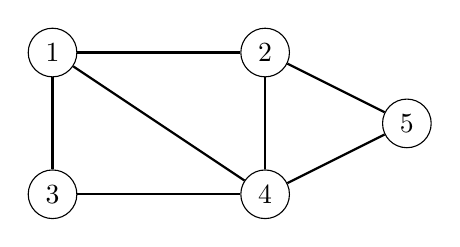
\begin{tikzpicture}[scale=0.9]
\node[draw, circle] (1) at (1,3) {$1$};
\node[draw, circle] (2) at (4,3) {$2$};
\node[draw, circle] (3) at (1,1) {$3$};
\node[draw, circle] (4) at (4,1) {$4$};
\node[draw, circle] (5) at (6,2) {$5$};

\path[draw,thick,-] (1) -- (2);
\path[draw,thick,-] (1) -- (3);
\path[draw,thick,-] (1) -- (4);
\path[draw,thick,-] (3) -- (4);
\path[draw,thick,-] (2) -- (4);
\path[draw,thick,-] (2) -- (5);
\path[draw,thick,-] (4) -- (5);
\end{tikzpicture}
\end{center}
一例は以下のとおりです。
\begin{center}
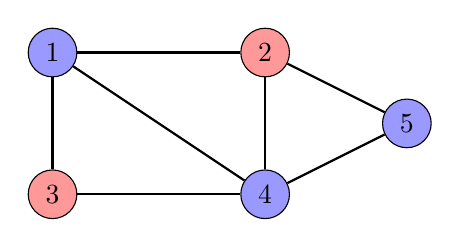
\begin{tikzpicture}[scale=0.9]
\node[draw, circle, fill=blue!40] (1) at (1,3) {$1$};
\node[draw, circle, fill=red!40] (2) at (4,3) {$2$};
\node[draw, circle, fill=red!40] (3) at (1,1) {$3$};
\node[draw, circle, fill=blue!40] (4) at (4,1) {$4$};
\node[draw, circle, fill=blue!40] (5) at (6,2) {$5$};

\path[draw,thick,-] (1) -- (2);
\path[draw,thick,-] (1) -- (3);
\path[draw,thick,-] (1) -- (4);
\path[draw,thick,-] (3) -- (4);
\path[draw,thick,-] (2) -- (4);
\path[draw,thick,-] (2) -- (5);
\path[draw,thick,-] (4) -- (5);
\end{tikzpicture}
\end{center}
このグラフには7本の辺があり、そのうち5本は両端の色が異なるので有効です。

この問題は有効な彩色が見つかるまでランダムに点を選ぶ生成するラスベガス・アルゴリズムを使って解けます。
各ノードの色は独立に選ばれ両方の色の確率が1/2になるようにします。

一つの辺の端点が異なる色になる確率は$1/2$なので、
端点の色が異なる辺の数の期待値は$m/2$です。
このため何度か試せば成立すると期待できます。
